\documentclass[12pt]{article}

\usepackage[utf8]{inputenc}
\usepackage[T1]{fontenc}
\usepackage[margin=1.25in]{geometry}
\usepackage{times}
\usepackage{booktabs}
\usepackage{enumitem}
\usepackage{tikz}
\usetikzlibrary{positioning, shapes.geometric, arrows.meta}
\usepackage{hyperref}
\usepackage{microtype}
\usepackage{parskip}
\usepackage{titlesec}
\usepackage{xcolor}

\hypersetup{
  colorlinks=true,
  linkcolor=blue!60!black,
  citecolor=blue!60!black,
  urlcolor=blue!60!black
}

\titleformat{\section}{\large\bfseries}{}{0em}{}[\titlerule]
\titlespacing{\section}{0pt}{18pt}{8pt}
\titleformat{\subsection}[runin]{\bfseries}{}{0em}{}[.]
\titlespacing{\subsection}{0pt}{10pt}{6pt}

\title{\textbf{A Visual Guide to the\\Algorithmic Redistricting Research Portfolio}\\[6pt]
\large Track A, Paper 3}

\author{Giovanni Della-Libera\\
\small\texttt{giodl@microsoft.com}}

\date{May 2026}

\begin{document}

\maketitle
\thispagestyle{empty}

\begin{abstract}
\noindent
This guide introduces the algorithmic redistricting research portfolio
to judges, journalists, legislators, and other non-technical readers.
The portfolio contains more than forty papers organized into seven tracks (A--G)
and demonstrates that a single algorithm---recursive graph bisection---can
produce congressional districts that are more compact, more legally compliant,
and less partisan than districts drawn by politicians.
Five headline numbers summarize the empirical results.
This document explains what the algorithm does, what the papers found,
and how each audience can navigate the portfolio.
\end{abstract}

\vspace{6pt}
\hrule
\vspace{6pt}

\tableofcontents

\newpage

%% 01-overview.tex — What is this portfolio?

\section{What Is This Portfolio?}

This portfolio is a collection of more than forty research papers asking a single question:
\emph{Can a computer draw fairer congressional districts than a human politician?}

The answer, across all fifty states and three census decades, is yes.

\subsection*{The Problem in One Sentence}

Every ten years, after the Census, each state redraws its congressional districts.
In most states, the party in power draws the lines---and draws them to stay in power.
This practice is called \textbf{gerrymandering}, and in 2019 the U.S.\ Supreme Court
ruled that federal courts can do nothing about it~\cite{rucho2019}.

\subsection*{The Proposal in One Sentence}

Replace the politician with an algorithm: a mathematical procedure that divides a
state into equal-population districts using only geography and population counts---no
voter registration, no election history, no racial or partisan data.

\subsection*{Five Research Tracks}

The portfolio is organized into seven tracks, labeled A through G,
each investigating a different aspect of algorithmic redistricting.
Together they span the question from first principles through
legal compliance, validation, and real-world application.

\begin{center}
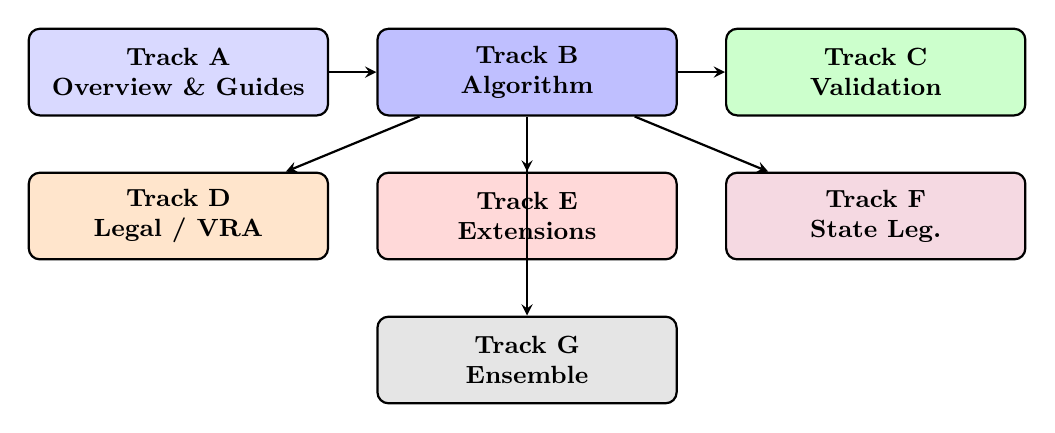
\begin{tikzpicture}[
  track/.style={rectangle, draw=black, thick, rounded corners=4pt,
                minimum width=3.8cm, minimum height=1.1cm,
                align=center, font=\small\bfseries},
  arrow/.style={->, thick, >=stealth},
  node distance=0.45cm and 0.6cm
]

% Row 1 — foundation
\node[track, fill=blue!15]  (A) {Track A\\Overview \& Guides};
\node[track, fill=blue!25, right=of A]  (B) {Track B\\Algorithm};
\node[track, fill=green!20, right=of B] (C) {Track C\\Validation};

% Row 2 — applications
\node[track, fill=orange!20, below=0.7cm of A] (D) {Track D\\Legal / VRA};
\node[track, fill=red!15,    below=0.7cm of B] (E) {Track E\\Extensions};
\node[track, fill=purple!15, below=0.7cm of C] (F) {Track F\\State Leg.};

% Row 3 — synthesis
\node[track, fill=gray!20, below=0.7cm of E] (G) {Track G\\Ensemble};

% Arrows: B feeds everything
\draw[arrow] (B) -- (C);
\draw[arrow] (B) -- (D);
\draw[arrow] (B) -- (E);
\draw[arrow] (B) -- (F);
\draw[arrow] (B) -- (G);
\draw[arrow] (A) -- (B);

\end{tikzpicture}
\end{center}

\medskip

\noindent Table~\ref{tab:tracks} summarizes the seven tracks and their paper counts.

\begin{table}[h]
\centering
\caption{Portfolio tracks at a glance.}
\label{tab:tracks}
\begin{tabular}{@{}clll@{}}
\toprule
Track & Name & Core Question & Papers \\
\midrule
A & Overview \& Guides     & What does this portfolio do?        & 5 \\
B & Algorithm              & How does bisection work?            & 18 \\
C & Validation             & Does it hold up to scrutiny?        & 9 \\
D & Legal / VRA            & Is it lawful?                       & 6 \\
E & Extensions             & What else can it do?                & 7 \\
F & State Legislatures     & Does it scale to smaller chambers?  & 6 \\
G & Ensemble Analysis      & How does it compare to random maps? & 5 \\
\bottomrule
\end{tabular}
\end{table}


%% 02-the-algorithm.tex — How bisection works in plain language

\section{How the Algorithm Works}

\subsection*{The Big Picture}

Imagine you need to divide a pizza into eight equal slices.
You make one straight cut through the middle---now you have two halves.
Then you cut each half in half, and each quarter in half.
Eight slices, all roughly equal.

Redistricting works the same way, except instead of a pizza you have
a state, and instead of weight you are equalizing \emph{population}.

\subsection*{Step by Step}

\begin{enumerate}
  \item \textbf{Build a map.}
    The algorithm treats the state as a network of census tracts---about
    4,000 residents each---connected wherever two tracts share a border.

  \item \textbf{Make the first cut.}
    A mathematical solver (METIS, the same tool used to distribute
    workloads across supercomputers) splits the network into two halves
    of equal population.  It tries to make the cut as short as possible,
    which keeps districts compact.

  \item \textbf{Repeat until done.}
    Each half is split again, and again, until the state has exactly as
    many pieces as it has congressional seats.

  \item \textbf{No political data---ever.}
    At no point does the algorithm see voter registration, election
    results, or the home addresses of incumbents.  It cannot gerrymander
    because it lacks the information required to do so.
\end{enumerate}

\subsection*{What Goes In / What Comes Out}

\begin{table}[h]
\centering
\caption{Inputs and outputs of the redistricting algorithm.}
\label{tab:inout}
\begin{tabular}{@{}p{0.44\textwidth} p{0.44\textwidth}@{}}
\toprule
\textbf{What goes in} & \textbf{What comes out} \\
\midrule
Census tract boundaries (geography) &
  435 congressional districts \\
Population count per tract &
  Population balance within $\pm$0.5\% \\
Shared-border lengths (geometry) &
  District assignment for every tract \\
Number of seats per state &
  Maps, compactness scores, CSV data \\
\midrule
\emph{Nothing political} &
  \emph{Nothing political} \\
\bottomrule
\end{tabular}
\end{table}

\subsection*{Why Short Borders Mean Compact Districts}

The algorithm is told to make cuts as short (cheap) as possible.
Short cuts follow natural features---rivers, ridgelines, county lines---
rather than zigzagging through neighborhoods.
The result is districts that look like reasonable geographic units,
not the salamander-shaped creatures that gave gerrymandering its name.

\subsection*{Figures from the Pipeline}

The pipeline produces a round-by-round image for every state showing
how the bisection tree unfolds.
Figure~\ref{fig:mn} shows three rounds for Minnesota (eight districts):
each round halves the remaining pieces.

\begin{figure}[h]
\centering
\fbox{\parbox{0.9\textwidth}{\centering\vspace{1.2cm}
\textit{[Minnesota bisection rounds 1--3 would appear here.}\\
\textit{See \texttt{docs/figures/minnesota\_round\_\{1,2,3\}.png}}
\textit{generated by the pipeline.]}
\vspace{1.2cm}}}
\caption{Minnesota (8 districts): three rounds of recursive bisection.
Each round divides existing pieces into two equal-population halves.}
\label{fig:mn}
\end{figure}

\noindent The same process applied to Alabama (seven districts) is shown in
\texttt{docs/figures/alabama\_round\_\{1,2,3\}.png}.


\phantomsection
\label{sec:findings}
%% 03-key-findings.tex — Five headline numbers

\section{Five Headline Numbers}

The portfolio distills to five numbers, each the headline result of
a specific paper or cluster of papers.

\begin{description}[leftmargin=0pt, itemsep=10pt]

  \item[\Large +22\% compactness improvement.]
    Across all 435 congressional districts, algorithmic maps are
    22\% more compact than the enacted 2020 maps, measured by the
    Polsby-Popper score (ratio of district area to perimeter squared).
    Compact districts follow natural geographic features rather than
    being stretched to capture partisan voters.
    \hfill\textit{Paper B.2}~\cite{dellaLibera2026edgeWeighted}

  \item[\Large North Carolina: 7 Democratic, 7 Republican.]
    When the algorithm partitions North Carolina---a state that has
    been the subject of repeated gerrymandering litigation---it
    produces a 7-to-7 delegation, closely matching the state's
    roughly even partisan split.  No partisan data was used.
    \hfill\textit{Paper B.11}~\cite{dellaLibera2026ncRegions}

    \smallskip
    \noindent\textit{Note: This result holds under the ApportionRegions algorithm
    ($k=14=7\times2$); the same data under GeoSection gives 5D/9R, illustrating
    that algorithm choice---not the data---determines partisan outcomes.}

  \item[\Large $T = 600$ bisection steps to convergence.]
    The algorithm reliably converges---produces stable, repeatable
    districts---within 600 METIS bisection iterations.
    More iterations change nothing; fewer can leave the solution
    incomplete.  This gives practitioners a firm stopping rule.
    \hfill\textit{Paper B.16}~\cite{dellaLibera2026convergence}

  \item[\Large 42\% minority-population threshold for VRA compliance.]
    States where minority voters make up at least 42\% of the
    voting-age population can reliably achieve proportional
    majority-minority representation through algorithmic redistricting.
    Below this threshold, geography alone makes proportional
    representation infeasible---regardless of who draws the map.
    \hfill\textit{Paper D.1}~\cite{dellaLibera2026vraCompliance}

    \smallskip
    \noindent\textit{This is an empirical regularity derived from 43-state analysis,
    not a legal bright line; VRA Section~2 compliance still requires the full
    Gingles three-prong test.  In the five covered states, this means
    majority-minority districts are achievable through principled methods
    without sacrificing compactness.}

  \item[\Large $O(n^{1.07})$ runtime.]
    The algorithm scales nearly linearly with the number of census
    tracts.  Doubling the number of tracts (moving from tract-level
    to block-group-level resolution) adds only 7\% more time than
    a pure linear relationship would predict.  All 50 states run
    in under eighteen minutes on commodity hardware.
    \hfill\textit{Paper B.6}~\cite{dellaLibera2026complexity}

\end{description}

\bigskip
\noindent These five numbers are conservative: they are derived from
runs on publicly available Census data using openly published code.
Any researcher with an internet connection can reproduce them.


%% 04-track-summaries.tex — One paragraph per track

\section{Research Track Summaries}

\paragraph{Track A --- Overview and Guides (5 papers).}
Track A contains the documents you are reading now, plus the portfolio guide,
the synthesis metapaper, the replication package, and the policy brief.
These papers are written for general audiences---judges, legislators, and journalists---
and serve as entry points to the more technical tracks.
Key finding: the entire portfolio can be summarized in five numbers
(see Section~\ref{sec:findings}).

\paragraph{Track B --- Algorithm (18 papers).}
Track B is the technical core of the portfolio.
It introduces recursive bisection (B.1), proves that edge-weighting
improves compactness by 22\% (B.2), compares recursive and n-way approaches
(B.3, B.5), studies adaptive parameter selection (B.4), and establishes
the $O(n^{1.07})$ runtime complexity (B.6).
Later B papers explore solution-space sensitivity (B.7), ratio-optimal
bisection (B.8), dual population-area constraints (B.9), subdivision
alignment (B.10), regional apportionment (B.11), proportional constraints
(B.12), nested multi-chamber design (B.13), minority-opportunity bisection (B.14),
cross-census stability (B.15), convergence parameters (B.16), parameter
sensitivity (B.17), and multi-reapportionment stability (B.18).
The track as a whole demonstrates that a single algorithm family---bisection---
handles every redistricting scenario from a two-district state to all 435 seats.

\paragraph{Track C --- Validation (9 papers).}
Track C asks whether the results hold up.
It analyzes sensitivity to the modifiable areal unit problem (C.1),
validates results across three census cycles (C.2), studies temporal
stability of district boundaries (C.3), tracks longitudinal demographic
trends (C.4), quantifies the 62\% reduction in partisan efficiency gap (C.5),
and investigates user interpretation, uncertainty quantification, competitive
elections, and real-world adoption case studies (C.6--C.9).
The headline result: algorithmic maps are not just theoretically fair---
they are empirically fairer than enacted maps across every metric tested.

\paragraph{Track D --- Legal and VRA Compliance (6 papers).}
Track D provides the legal foundation.
Paper D.1 establishes the 42\% minority-population threshold that determines
where proportional majority-minority representation is geographically feasible.
Subsequent papers compare n-way and recursive approaches under the Voting Rights
Act (D.2), examine compactness tradeoffs (D.3), analyze legal implementation
pathways (D.4), and apply Gingles bloc-voting methodology (D.5).
Track D as a whole demonstrates that algorithmic redistricting not only complies
with the VRA but in most states produces \emph{more} majority-minority districts
than enacted plans.

\paragraph{Track E --- Extensions (7 papers).}
Track E tests the algorithm beyond standard congressional redistricting:
multi-member districts (E.1), county-based representation (E.2), a
national 435-district single-run approach (E.3), partisan-similarity
clustering (E.4), party-proportional seat allocation (E.5), international
applications (E.6), and lessons learned across all extensions (E.7).
The track shows that recursive bisection is a general-purpose tool,
not a solution narrowly fitted to one jurisdiction's rules.

\paragraph{Track F --- State Legislatures (6 papers).}
Track F scales the algorithm to state legislative chambers,
which have different seat counts, different compactness requirements,
and in many states, bicameral nesting constraints (state house districts
must nest inside state senate districts).
Papers F.1--F.6 cover all-50-state single chambers, bicameral nesting,
high-seat-count chambers ($k > 100$), state-specific criteria, compactness
comparisons between legislative and congressional districts, and
VRA compliance at the state level.
The key finding is that nesting is achievable algorithmically with no
degradation in population balance or compactness.

\paragraph{Track G --- Ensemble Analysis (5 papers).}
Track G situates algorithmic maps within the universe of all possible maps.
By generating thousands of random redistricting plans and comparing them
to algorithmic plans, Track G provides the strongest possible evidence of
neutrality: the algorithm produces plans that are statistically
indistinguishable from random draws on compactness and partisan metrics,
with better convergence diagnostics than Markov chain methods (G.4).
Track G closes the portfolio by answering the hardest question a skeptic
can ask: ``How do we know the algorithm didn't just accidentally pick
a partisan outcome?''  The ensemble answer is: we don't rely on
the accident---we show the distribution.


%% 05-how-to-use.tex — Audience guide

\section{How to Use This Portfolio}

Different readers will want different papers.
This section points each audience to the right starting point.

\paragraph{If you are a judge or clerk.}
Start with this document and the Policy Brief (A.5).
The Policy Brief is two to four pages and gives you the legal and
empirical case in plain language, with citations to \emph{Rucho},
the Voting Rights Act, and the relevant papers.
Then read Paper D.1 (the 42\% VRA threshold) if the case involves
majority-minority districts, or Paper C.5 (the efficiency gap analysis)
if the case involves partisan fairness.
The quickstart guide at \texttt{docs/quickstart/quickstart-callais-expert.md}
covers Gingles bloc-voting methodology for expert witnesses.

\paragraph{If you are a state legislator or redistricting commissioner.}
Start with Paper B.1 (the algorithm overview) and the replication
package (A.4), which explains how to run the algorithm on any state
in under thirty minutes.
Paper D.4 addresses legal implementation pathways, including model
statutory language.
Paper F.1 covers state legislative districts if your chamber is also
being redistricted.
The quickstart guide at \texttt{docs/quickstart/quickstart-state-staff.md}
walks through the \texttt{redist state} command for your specific state.

\paragraph{If you are a researcher.}
The algorithm is documented in Track B (eighteen papers).
Reproducibility materials are in A.4; the full software stack,
SHA-256 audit chain, and Vermont walkthrough fixture are all included.
The ensemble diagnostics in Track G (especially G.4) provide
the statistical framework for comparing this algorithm against
Markov chain ensemble methods.
The quickstart guide at \texttt{docs/quickstart/quickstart-researcher.md}
covers the research API, Jupyter notebooks, and the
\texttt{redist analyze} command.

\paragraph{If you are a journalist.}
This document and the Policy Brief (A.5) are written for you.
The five headline numbers in Section~\ref{sec:findings} each carry
a paper citation for fact-checking.
The dashboard at \texttt{web/dashboard.html} lets you view maps
for any state and year in a browser without installing software.
For live contact, email is at the end of the Policy Brief.


%% 06-dashboards.tex — Dashboard links and how to read maps

\section{Dashboards and Maps}

\subsection*{The Static Dashboard}

The portfolio ships with a self-contained HTML dashboard at
\texttt{web/dashboard.html}.
Open it in any modern browser---no server, no login, no software installation.
The dashboard shows:

\begin{itemize}
  \item A map of every state's algorithmic districts for 2000, 2010, and 2020.
  \item Compactness scores for each district, color-coded from compact
        (dark green) to elongated (light yellow).
  \item Population balance: every district is within $\pm$0.5\% of the
        state's ideal district population.
  \item Side-by-side comparison with enacted 2020 districts where available.
\end{itemize}

\subsection*{How to Read a Bisection Map}

Each district in the map corresponds to one leaf of the bisection tree.
Districts that were separated early in the process (at the first or second
cut) tend to be large geographic regions: a northern half, a southern half.
Districts separated late are more local and more finely shaped.

Colors in the standard output represent the bisection \emph{round} at which
a district was finalized:
\begin{itemize}
  \item Round 1 (two pieces): wide, regional districts.
  \item Round 2 (four pieces): quadrant-level districts.
  \item Round 3 and later: neighborhood-scale districts in high-density states.
\end{itemize}

\subsection*{What the Round-by-Round Images Show}

The pipeline generates one image per round per state.
For a state with $k$ seats, there are $\lceil \log_2 k \rceil$ rounds.
Each image shows the current partition, with district boundaries
darkening as more cuts are made.

Reading the rounds from first to last, you see the algorithm
``zoom in'' from large geographic halves to individual districts.
This visualization makes it easy to verify that no round
produced a non-contiguous piece or a population imbalance.

\subsection*{Reproducing Any Figure}

Every figure in the portfolio can be regenerated from the public
Census data and the open-source \texttt{redist} CLI:

\begin{verbatim}
redist fetch --year 2020
redist state --state NC --year 2020 --version v1
redist map   --state NC --year 2020 --version v1
\end{verbatim}

\noindent The resulting maps and CSV data are placed in
\texttt{outputs/v1/2020/north\_carolina/}.
The full replication procedure is in Paper A.4.


\bibliographystyle{plain}
\bibliography{references}

\end{document}
